\ExamPart{Câu trắc nghiệm trả lời ngắn}{2}{}

\NQuestion Tìm tổng các nghiệm nguyên của bất phương trình $(x-2)(x-5)<0$.

\NQuestion Trong mặt phẳng tọa độ $Oxy$, đường thẳng đi qua hai điểm $A(1;2)$ và $B(3;6)$ có phương trình dạng $y=kx+b$. Tính giá trị $k+b$.

\NQuestion Từ 4 học sinh nam và 3 học sinh nữ, có bao nhiêu cách chọn ra 2 học sinh sao cho có ít nhất 1 học sinh nữ?

\NQuestion Một cổng vòm có dạng nửa elip như hình vẽ, với phương trình $\dfrac{x^2}{16}+\dfrac{y^2}{9}=1$ $(y\ge 0)$. Tính chiều cao của cổng tại điểm cách tâm $2$m theo phương ngang (làm tròn đến hàng phần mười).

\begin{center}
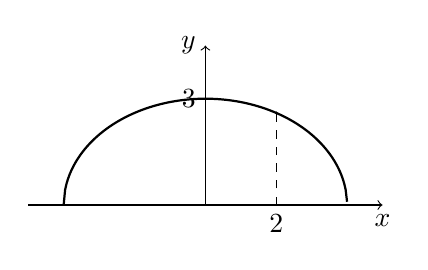
\begin{tikzpicture}[scale=0.45]
    \draw[->] (-5,0) -- (5,0) node[below] {$x$};
    \draw[->] (0,0) -- (0,4.5) node[left] {$y$};

    \draw[thick, domain=-4:4, samples=200] plot (\x,{3*sqrt(1-\x*\x/16)});
    \draw[thick] (-4,0) -- (4,0);

    \draw[dashed] (2,0) -- (2,{3*sqrt(1-4/16)});
    \fill (2,{3*sqrt(1-4/16)}) circle (1.2pt);

    \node[below] at (2,0) {$2$};
    \node[left] at (0,3) {$3$};
\end{tikzpicture}

\end{center}
